\documentclass{article}
\date{} % Remove a exibição da data
\usepackage{xcolor}
\usepackage{listings}
\usepackage{graphicx}

\lstset{
  language=C,
  basicstyle=\ttfamily,
  keywordstyle=\bfseries\color{blue},
  commentstyle=\color{gray},
  stringstyle=\color{red!70!black},
  numberstyle=\tiny,
  stepnumber=1,
  numbersep=5pt,
  backgroundcolor=\color{white},
  breaklines=true,
  breakautoindent=true,
  showspaces=false,
  showstringspaces=false,
  showtabs=false,
  tabsize=2
}




\title{Trabalho microcontroladores 1}
\author{Marco Antonio}

\begin{document}

\maketitle

\section{Introdução}

Esse relatorio é relativo ao trabalho 1 de microcontroladores, visando explicar
o funcionamento do projeto relativo ao trabalho

\section{defines}
nessa seção estão as defines necessarias para o codigo funcionar assim
como os include da gpio , interrupt, sistick , contidas na driverlib


\begin{lstlisting}

#include <stdint.h>
#include <stdio.h>
#include <stdbool.h>

#define ESC_REG(x)                  (*((volatile uint32_t *)(x)))

#define SYSCTL_RCGC2_R              0x400FE108
#define GPIO_BASE         0x400FE000
#define GPIO_OFFSET       0x608

#define PORTAL_A          0x00000001 // 0000 0001 em binario
#define PORTAL_B          0x00000002 // 0000 0010 em binario
#define PORTAL_C          0x00000004 // 0000 0100 em binario
#define PORTAL_D          0x00000008 // 0000 1000 em binario
#define PORTAL_E          0x00000010 // 0001 0000 em binario
#define PORTAL_F          0x00000020 // 0010 0000 em binario

#define PORTAL_A_BASE 0x40004000
#define PORTAL_B_BASE 0x40005000
#define PORTAL_C_BASE 0x40006000
#define PORTAL_D_BASE 0x40007000
#define PORTAL_E_BASE 0x40024000
#define PORTAL_F_BASE 0x40025000

#define PINO_0            0x01
#define PINO_1            0x02
#define PINO_2            0x04
#define PINO_3            0x08
#define PINO_4            0x10
#define PINO_5            0x20
#define PINO_6            0x40
#define PINO_7            0x80

#define GPIO_O_GPIODIR    0x400
#define GPIO_O_GPIODEN    0x51C // digital ou outra funcao
#define GPIO_O_GPIODR2R   0x500
#define GPIO_O_GPIODR4R   0x504
#define GPIO_O_GPIODR8R   0x508
#define GPIO_O_GPIOSLR    0x500
#define GPIO_O_GPIOPUR    0x510
#define GPIO_O_DATA_R     0x000
#define GPIO_O_GPIOLOCK   0x520
#define GPIO_O_GPIOCR     0x524

#define DELAY_BASE 1000000  // 1000000 = 2.5 segundos, aproximadamente
//#define DELAY DELAY_BASE/(60*2.5) // piscar 60 vezes por segundo
#define DELAY 10000000
#define GPIO_PORTF_LOCK_R (*((volatile uint32_t *)0x40025520))
#define GPIO_PORTF_CR_R (*((volatile uint32_t *)0x40025524))

#include "driverlib/gpio.h"
#include "inc/hw_memmap.h"
#include "inc/hw_gpio.h"
#include "inc/hw_ints.h"
#include "driverlib/gpio.h"
#include "driverlib/interrupt.h"
#include "driverlib/sysctl.h"

int v;
int s = 0

\end{lstlisting}

\section{Funçôes}

\subsection{Funções de ativação display}
nessa seção estão as funções de ativação do display de sete segmentos

\begin{lstlisting}
void habilita_portal2(uint32_t portal) {
    ESC_REG(GPIO_BASE + GPIO_OFFSET)  |= portal;
}

void habilita_portal(uint32_t portal){
    ESC_REG(SYSCTL_RCGC2_R) |= portal;
}

void desabilita_portal(uint32_t portal){
    ESC_REG(SYSCTL_RCGC2_R) &= ~(portal);
}

void configura_pino_saida(uint32_t portal_base, uint8_t pino){
    ESC_REG(portal_base + GPIO_O_GPIODIR)  |= pino;
    ESC_REG(portal_base + GPIO_O_GPIODEN)  |= pino;
    ESC_REG(portal_base + GPIO_O_GPIODR2R) |= pino;
    ESC_REG(portal_base + GPIO_O_GPIODR4R) &= ~(pino);
    ESC_REG(portal_base + GPIO_O_GPIODR8R) &= ~(pino);
    ESC_REG(portal_base + GPIO_O_GPIOSLR) &= ~(pino);
}

void escrita_pinos(uint32_t portal_base, uint8_t pino, uint8_t valor) {
    ESC_REG (portal_base + (GPIO_O_DATA_R + (pino << 2))) = valor;
}

void limpa_display(){
    escrita_pinos(PORTAL_C_BASE, PINO_6 | PINO_5 | PINO_4, 0x00);
    escrita_pinos(PORTAL_E_BASE, PINO_3 | PINO_2 | PINO_1 | PINO_0, 0x00);

    escrita_pinos(PORTAL_B_BASE, PINO_6 , 0x00);
    escrita_pinos(PORTAL_B_BASE, PINO_7,  0x00);
    escrita_pinos(PORTAL_D_BASE, PINO_2 , 0x00);
    escrita_pinos(PORTAL_D_BASE, PINO_3,  0x00);
}
void  delay(uint32_t delayms){
    SysCtlDelay(delayms);

}



// Da um delay no sistema, sem uma unidade definida(segundo, millisegundo, etc),
// onde o valor foi definido na pratica
/*void delay(uint32_t i){
    uint32_t cont;
    for(cont = 0; cont < i; cont++) {}
}

\end{lstlisting}

\subsection{ Funções de configuração display}

A segunda parte de codigo envolve funções básica para o display de 7 segmentos. escritapinos() ,habilitaportal() , desabilitaportal() ,limpadisplay(), delay(),configura os pinos passados como saída,a escrita pino escreve nos pino especificados que são justamente os conectados ao display de  segmentos, e limpa  display, limpa o display apos execução.
Essa parte se refere a escolha dos dígitos de acordo como passar do tempo. Acende os dígitos de acordo como forem chamados, e quadradocima() e quadradobaixo() para os quadrados nos segmentos superiores e inferiores. 


\begin{lstlisting}

// Escolhe o digito que vai ser feita a escrita do numero
//PORTA B PINO 6, PINO 7
//PORTA D PINO 3 , PINO 2
void escolhe_digito(uint32_t num) {
    switch(num){
    case 1:
        escrita_pinos(PORTAL_B_BASE, PINO_6 , 0X00);
        escrita_pinos(PORTAL_B_BASE, PINO_7,  PINO_7);
        escrita_pinos(PORTAL_D_BASE, PINO_3 , PINO_3);
        escrita_pinos(PORTAL_D_BASE, PINO_2,  PINO_2);
        break;
    case 2:
        escrita_pinos(PORTAL_B_BASE, PINO_6 , PINO_6);
        escrita_pinos(PORTAL_B_BASE, PINO_7,  0X00);
        escrita_pinos(PORTAL_D_BASE, PINO_2 , PINO_2);
        escrita_pinos(PORTAL_D_BASE, PINO_3,  PINO_3);
        break;
    case 3:
        escrita_pinos(PORTAL_B_BASE, PINO_7 , PINO_7);
        escrita_pinos(PORTAL_B_BASE, PINO_6,  PINO_6);
        escrita_pinos(PORTAL_D_BASE, PINO_2 , 0X00);
        escrita_pinos(PORTAL_D_BASE, PINO_3,  PINO_3);
        break;
    case 4:
        escrita_pinos(PORTAL_B_BASE, PINO_6 , PINO_6);
        escrita_pinos(PORTAL_B_BASE, PINO_7,  PINO_7);
        escrita_pinos(PORTAL_D_BASE, PINO_2 , PINO_2);
        escrita_pinos(PORTAL_D_BASE, PINO_3,  0x00);
        break;
    }
}


void quadrado_cima(){
        escrita_pinos(PORTAL_C_BASE, PINO_5| PINO_6 ,PINO_5 + PINO_6 );
        escrita_pinos(PORTAL_E_BASE,  PINO_1| PINO_0,  PINO_1 + PINO_0);


    }

void quadrado_baixo(){
    escrita_pinos(PORTAL_C_BASE,  PINO_4|PINO_6 , PINO_4 + PINO_6);
    escrita_pinos(PORTAL_E_BASE, PINO_3 | PINO_2, PINO_3 + PINO_2);


    }

    void escreve_quadrado()
    {
        uint32_t sent_h[8] = {1,2,3,4,4,3,2,1};
        uint32_t i = 0;
        for (i = 0;i < 4; i++){
              limpa_display();
              escolhe_digito(sent_h[i]);
              quadrado_cima();
              delay(10000000);
        }

        for (i = 4;i < 8; i++){
              limpa_display();
              escolhe_digito(sent_h[i]);
              quadrado_baixo();
              delay(10000000);
        }

    }



    void escreve_quadrado_vel(uint32_t vel) {

        uint32_t sent_h[8] = {1,2,3,4,4,3,2,1};
                uint32_t i = 0;
                for (i = 0;i < 4; i++){
                      limpa_display();
                      escolhe_digito(sent_h[i]);
                      quadrado_cima();
                      delay(vel);
                }

                for (i = 4;i < 8; i++){
                      limpa_display();
                      escolhe_digito(sent_h[i]);
                      quadrado_baixo();
                      delay(vel);
                }

      }
    void set_vel(int v)
    {
    uint32_t vel = 0;
    switch(v)
        {
        case 0:
            escreve_quadrado();
            break;
        case 1:
            vel = 1000000;
            escreve_quadrado_vel(vel);
            break;
        case 2:
            vel = 500000;
            escreve_quadrado_vel(vel);
            break;
        case 3:
            vel =250000;
            escreve_quadrado_vel(vel);
            break;
        }
    }
    void escreve_quadrado_anti() {
/*
            uint32_t sent_a[8] = {1,2,3,4,4,3,2,1};
            uint32_t i = 0;


            for (i = 1;i < 4; i--){
                  limpa_display();
                  escolhe_digito(sent_a[i]);
                  quadrado_baixo();
                  delay(5000000);
            }
            for (i = 4;i < 8; i--){
                 limpa_display();
                 escolhe_digito(sent_a[i]);
                 quadrado_cima();
                 delay(5000000);
           }
           */
            limpa_display();
            escolhe_digito(1);
            quadrado_baixo();
            delay(DELAY);

            limpa_display();
            escolhe_digito(2);
            quadrado_baixo();
            delay(DELAY);

            limpa_display();
            escolhe_digito(3);
            quadrado_baixo();
            delay(DELAY);

            limpa_display();
            escolhe_digito(4);
            quadrado_baixo();
            delay(DELAY);

            limpa_display();
           escolhe_digito(4);
           quadrado_cima();
           delay(DELAY);

           limpa_display();
           escolhe_digito(3);
           quadrado_cima();
           delay(DELAY);

          limpa_display();
          escolhe_digito(2);
          quadrado_cima();
          delay(DELAY);

          limpa_display();
          escolhe_digito(1);
          quadrado_cima();
          delay(DELAY);

    }

    void escreve_quadrado_anti_vel(uint8_t vel) {
        /*
               uint32_t sent_a[8] = {1,2,3,4,4,3,2,1};
               uint32_t i = 0;
               for (i = 4;i > 0; i--){
                     limpa_display();
                     escolhe_digito(sent_a[i]);
                     quadrado_cima();
                     delay(vel);
               }

               for (i = 8;i > 4; i--){
                     limpa_display();
                     escolhe_digito(sent_a[i]);
                     quadrado_baixo();
                     delay(vel);
               }
               */
        limpa_display();
        escolhe_digito(1);
        quadrado_baixo();
        delay(vel);

        limpa_display();
        escolhe_digito(2);
        quadrado_baixo();
        delay(vel);

        limpa_display();
        escolhe_digito(3);
        quadrado_baixo();
        delay(vel);

        limpa_display();
        escolhe_digito(4);
        quadrado_baixo();
        delay(vel);

        limpa_display();
       escolhe_digito(4);
       quadrado_cima();
       delay(vel);

       limpa_display();
       escolhe_digito(3);
       quadrado_cima();
       delay(vel);

      limpa_display();
      escolhe_digito(2);
      quadrado_cima();
      delay(vel);

      limpa_display();
      escolhe_digito(1);
      quadrado_cima();
      delay(vel);

}

    void set_vel_anti(int v)
       {
       uint32_t vel = 0;
       switch(v)
           {
           case 0:
               escreve_quadrado_anti();
               break;
           case 1:
               vel = 1000000;
               escreve_quadrado_anti_vel(vel);
               break;
           case 2:
               vel = 500000;
               escreve_quadrado_anti_vel(vel);
               break;
           case 3:
               vel =250000;
               escreve_quadrado_anti_vel(vel);
               break;
           }
       }

\end{lstlisting}
\subsection{Funções de  configuração interrupts e sistick}
Essa parte configura as interrupções, e acende o led vermelho se sw1 for apertado, e modifica a velocidade.Se a sw2  for apertado,
vai ser modificado o sentido de rotação do display 
\begin{lstlisting}
    void PortFIntHandler(void)
{
    GPIOIntClear(GPIO_PORTF_BASE, GPIO_PIN_0);
    GPIOIntClear(GPIO_PORTF_BASE, GPIO_PIN_4);

    if(!(GPIOPinRead(GPIO_PORTF_BASE, GPIO_PIN_0) & GPIO_PIN_0)){
        GPIOPinWrite(GPIO_PORTF_BASE, GPIO_PIN_1, GPIO_PIN_1);

                    if(v==4){
                        v = 0;
                    } else{
                        v++;
                    }
                    set_vel(v);

                 }

    if(!(GPIOPinRead(GPIO_PORTF_BASE, GPIO_PIN_4) & GPIO_PIN_4))
       {
        GPIOPinWrite(GPIO_PORTF_BASE, GPIO_PIN_2, GPIO_PIN_2);
                 if(s == 1){
                  set_vel_anti(v);
                 } else {
                     set_vel(v);
                     s = 0;
                 }
                 s++;
    }
}

\end{lstlisting}

\section{main}
Na main está habilitado as portas referentes ao display de sete segmentos, e configura os pinos de saída conectados ao display.


\begin{lstlisting}
int main(){
    volatile uint32_t ui32Loop;

       // Habilita os portais relativos aos pinos do display
       habilita_portal(PORTAL_B);
       habilita_portal(PORTAL_D);
       habilita_portal(PORTAL_C);
       habilita_portal(PORTAL_E);
       // Faz leitura dummy para efeito de atraso
       ui32Loop = ESC_REG(SYSCTL_RCGC2_R);

       configura_pino_saida(PORTAL_C_BASE, PINO_6 | PINO_5 | PINO_4);
       configura_pino_saida(PORTAL_E_BASE, PINO_3 | PINO_2 | PINO_1 | PINO_0);
       configura_pino_saida(PORTAL_D_BASE, PINO_3 | PINO_2);
       configura_pino_saida(PORTAL_B_BASE, PINO_6 | PINO_7);

       SysCtlClockSet(SYSCTL_SYSDIV_5|SYSCTL_USE_PLL|SYSCTL_XTAL_16MHZ|SYSCTL_OSC_MAIN);
      
       SysCtlPeripheralEnable(SYSCTL_PERIPH_GPIOF);
       configura_pino_saida(PORTAL_F_BASE, PINO_1 | PINO_2| PINO_3);
       GPIO_PORTF_LOCK_R = 0x4C4F434B;
       GPIO_PORTF_CR_R = 0x1F;
       GPIOPinTypeGPIOInput(GPIO_PORTF_BASE, GPIO_PIN_4|GPIO_PIN_0);
       GPIOPadConfigSet(GPIO_PORTF_BASE,GPIO_PIN_0|GPIO_PIN_4, GPIO_STRENGTH_2MA,GPIO_PIN_TYPE_STD_WPU);

       IntMasterEnable();
       IntEnable(INT_GPIOF);
       GPIOIntTypeSet(GPIO_PORTF_BASE, GPIO_PIN_0,GPIO_FALLING_EDGE);
       GPIOIntEnable(GPIO_PORTF_BASE, GPIO_INT_PIN_0);

       GPIOIntTypeSet(GPIO_PORTF_BASE, GPIO_PIN_4,GPIO_FALLING_EDGE);
       GPIOIntEnable(GPIO_PORTF_BASE, GPIO_INT_PIN_4);


       // Loop principal
       while(1)
       {

             //uint32_t v = 0;
             // se o sw2 for acionado
//             if(!(GPIOPinRead(GPIO_PORTF_BASE, GPIO_PIN_0) & GPIO_PIN_0)){
//                if(v==3){
//                    v = 0;
//                } else{
//                    v++;
//                }
//                set_vel(v);
//
//             }
             //se sw1 for acionado
             /*
             if(!(GPIOPinRead(GPIO_PORTF_BASE, GPIO_PIN_4) & GPIO_PIN_4))
             {
                 uint8_t s = 1;
                 if (s == 2){
                     s = 1;
                     escreve_quadrado();

                 } else{
                     s++;

                 }
             
           }
       }
    
\end{lstlisting}


\begin{figure}
   \centering
  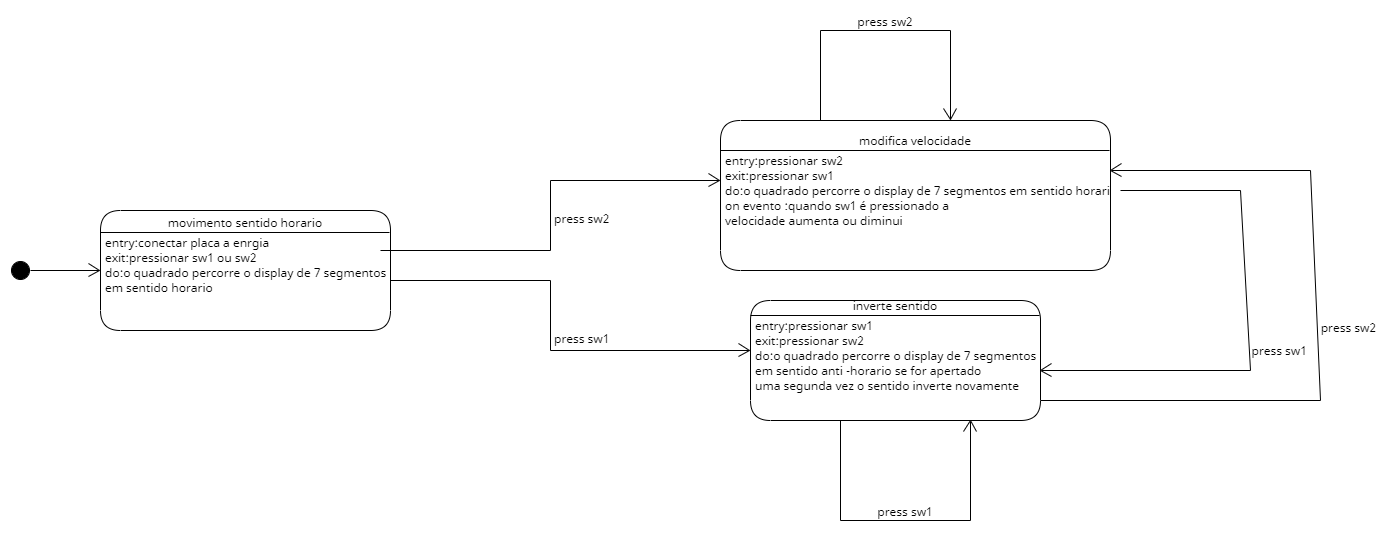
\includegraphics[width=1.3\textwidth]{digrama.png}
  \caption{Diagrama Estados finitos}
  \label{fig:diagrama}
\end{figure}



\end{document}




